% Template for ICIP-2013 paper; to be used with:
%          spconf.sty  - ICASSP/ICIP LaTeX style file, and
%          IEEEbib.bst - IEEE bibliography style file.
% --------------------------------------------------------------------------
\documentclass{article}
\usepackage{spconf,amsmath,graphicx}
\usepackage[frenchb]{babel}
\usepackage[utf8]{inputenc}
\usepackage{graphicx}

% Example definitions.
% --------------------
\def\x{{\mathbf x}}
\def\L{{\cal L}}

% Title.
% ------
\title{IDENTIFICATION ET COMPTAGE DE PI\'{E}TONS}
%
% Single address.
% ---------------
%\name{Author(s) Name(s)\thanks{Thanks to XYZ agency for funding.}}
%\address{Author Affiliation(s)}
%


\name{Berta Bescos \qquad Julien Guichon \qquad Dimitri Gominski \qquad}

\address{}
	
\begin{document}
%\ninept
%
\maketitle
%
\begin{abstract}
	
	The range of pedestrian detection techniques, in order to achieve better performance and efficiency, is getting more and more complex, and thus the implementation of these algorithms can become time-consuming in conception phase.
	
	By using 2 different approaches, we demonstrate the impact of acquisition context on the performance of these methods, and study the viability of a "naive" algorithm versus a modern version of object identification applied to pedestrian detection.
\end{abstract}
%

%
\section{Introduction}
\label{sec:intro}
	Le développement de techniques fiables pour la détection de piétons dans les systèmes numériques est une problématique récente, et porteuse d'enjeux pour de nombreux domaines tels que la sécurité, la robotique, la maîtrise des flux humains en urbanisme... 

	Le coeur de la chaîne de traitement visant à associer à une zone spécifique de l'image une classe (piéton/non-piéton) repose sur 2 opérations élémentaires : la description et la décision. La description extrait des caractéristiques de ladite zone en fournissant des valeurs numériques caractérisant la forme, l'intensité et la texture. De cette manière on associe un ensemble d'informations quantifiées à un objet pour l'instant non-identifié. La décision, en synthétisant toutes ces valeurs numériques, donne un résultat binaire sur l'appartenance de l'objet à une classe.

	Il va de soi que l'exhaustivité des descripteurs et la précision des classifieurs (organes de décision) sont la clé d'algorithmes infaillibles, mais elles se traduisent invariablement par plus de complexité, et si des précautions ne sont pas prises, par un temps de calcul allongé. Le choix du descripteur et du classifieur est un sujet sensible à de nombreuses contraintes, et dépend fortement des données disponibles pour la conception, des conditions d'utilisation de l'algorithme, et des performances attendues. L'étude des différents descripteurs et classifieurs s'est faite de manière empirique dans les 20 dernières années, et une large bibliographie est disponible pour les caractériser et préciser les conditions dans lesquels ils fournissent les meilleurs résultats.

	Ce rapport décrit les performances obtenues avec 2 algorithmes courants tirés de 2 approches différentes du problème de l'identification et du comptage d'un flux épars de piétons.

\section{\'{E}TUDE BIBLIOGRAPHIQUE CHRONOLOGIQUE}
\label{sec:format}

	Dès 1985, T. Tsukiyama et Y. Shirai [5] ont proposé une technique rudimentaire d'identification humaine en travaillant avec l'intensité pixel par pixel.

	En 1997 est proposée au MIT [4] une technique innovante de description des formes basée sur les ondelettes de Haar, associée à un classifieur SVM. L'idée de séparer descripteur et classifieur est depuis devenue un standard dans ce domaine.

	En 1998, cette technique est perfectionnée [6] pour la rendre universelle en incluant un apprentissage le plus complet possible avec un set de données dédiées, pour permettre l'exécution dans des conditions variées. L'article introduit également la notion d'échelle variable pour la fenêtre de détection.

	Dalal \& Triggs [2] publient en 2005 un article de référence dans le domaine (+6000 citations). Ils expliquent une méthode complète, d'implémentation relativement simple, pour mettre en place une chaîne de détection de performances correctes. Leur méthode repose sur l'histogramme des gradients orientés pour décrire la forme d'un piéton, et la décision se fait avec une SVM (support vector machine) linéaire.

	Depuis, de nombreuses nouvelles approches ont été proposées, citons entre autres l'utilisation des informations de couleur [8], du mouvement [10], du bootstrapping (réutilisation des résultats, re-training) [8], de très larges sets de données d'apprentissages acquises par data-mining [11]  \textit{etc.}, avec la problématique du temps de calcul toujours au coeur du problème [9].


\section{CONTEXTE}
\label{sec:pagestyle}

	Dans le cadre de l'étude de faisabilité d'un algorithme de détection en temps réel à 95\% de précision, nous disposons d'un set de données d'entrées dans des conditions relativement favorables (voir Figure 1). La caméra fournissant ces images est fixe, les seuls évènements d'occlusion concernent les croisements de piétons, et la zone concernée est une section de route fréquentée uniquement par des piétons, ce qui limite les risques de confusion avec du mobilier urbain ou des véhicules. Les seules contraintes sont l'orientation légèrement verticale de la caméra (ce qui limite la surface identifiable du corps humain) et la profondeur de champ qui implique de devoir gérer les changements d'échelle.
	
	\begin{figure}
		\begin{center}			
			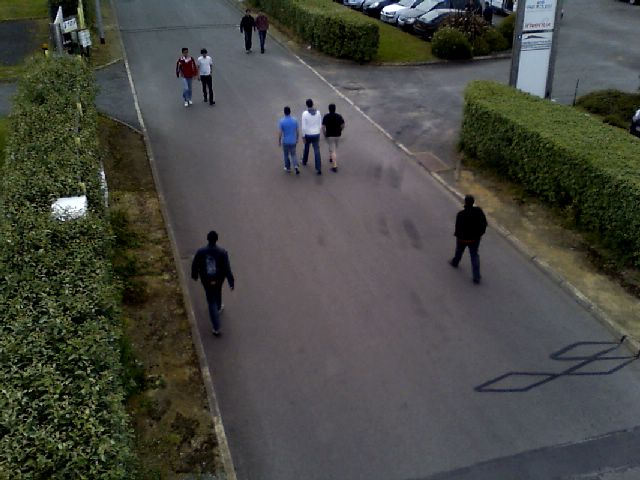
\includegraphics[scale=0.3]{Img/detection_0156}
		\end{center}
		\caption{Données d'entrée}
	\end{figure}

\section{TYPE-STYLE AND FONTS}
\label{sec:typestyle}

To achieve the best rendering both in printed proceedings and electronic proceedings, we
strongly encourage you to use Times-Roman font.  In addition, this will give
the proceedings a more uniform look.  Use a font that is no smaller than nine
point type throughout the paper, including figure captions.

In nine point type font, capital letters are 2 mm high.  {\bf If you use the
smallest point size, there should be no more than 3.2 lines/cm (8 lines/inch)
vertically.}  This is a minimum spacing; 2.75 lines/cm (7 lines/inch) will make
the paper much more readable.  Larger type sizes require correspondingly larger
vertical spacing.  Please do not double-space your paper.  TrueType or
Postscript Type 1 fonts are preferred.

The first paragraph in each section should not be indented, but all the
following paragraphs within the section should be indented as these paragraphs
demonstrate.

\section{MAJOR HEADINGS}
\label{sec:majhead}

Major headings, for example, "1. Introduction", should appear in all capital
letters, bold face if possible, centered in the column, with one blank line
before, and one blank line after. Use a period (".") after the heading number,
not a colon.

\subsection{Subheadings}
\label{ssec:subhead}

Subheadings should appear in lower case (initial word capitalized) in
boldface.  They should start at the left margin on a separate line.
 
\subsubsection{Sub-subheadings}
\label{sssec:subsubhead}

Sub-subheadings, as in this paragraph, are discouraged. However, if you
must use them, they should appear in lower case (initial word
capitalized) and start at the left margin on a separate line, with paragraph
text beginning on the following line.  They should be in italics.

\section{PRINTING YOUR PAPER}
\label{sec:print}

Print your properly formatted text on high-quality, 8.5 x 11-inch white printer
paper. A4 paper is also acceptable, but please leave the extra 0.5 inch (12 mm)
empty at the BOTTOM of the page and follow the top and left margins as
specified.  If the last page of your paper is only partially filled, arrange
the columns so that they are evenly balanced if possible, rather than having
one long column.

In LaTeX, to start a new column (but not a new page) and help balance the
last-page column lengths, you can use the command ``$\backslash$pagebreak'' as
demonstrated on this page (see the LaTeX source below).

\section{PAGE NUMBERING}
\label{sec:page}

Please do {\bf not} paginate your paper.  Page numbers, session numbers, and
conference identification will be inserted when the paper is included in the
proceedings.

\section{ILLUSTRATIONS, GRAPHS, AND PHOTOGRAPHS}
\label{sec:illust}

Illustrations must appear within the designated margins.  They may span the two
columns.  If possible, position illustrations at the top of columns, rather
than in the middle or at the bottom.  Caption and number every illustration.
All halftone illustrations must be clear black and white prints.  Colors may be
used, but they should be selected so as to be readable when printed on a
black-only printer.

Since there are many ways, often incompatible, of including images (e.g., with
experimental results) in a LaTeX document, below is an example of how to do
this \cite{Lamp86}.

\section{FOOTNOTES}
\label{sec:foot}

Use footnotes sparingly (or not at all!) and place them at the bottom of the
column on the page on which they are referenced. Use Times 9-point type,
single-spaced. To help your readers, avoid using footnotes altogether and
include necessary peripheral observations in the text (within parentheses, if
you prefer, as in this sentence).

% Below is an example of how to insert images. Delete the ``\vspace'' line,
% uncomment the preceding line ``\centerline...'' and replace ``imageX.ps''
% with a suitable PostScript file name.
% -------------------------------------------------------------------------
\begin{figure}[htb]

\begin{minipage}[b]{1.0\linewidth}
  \centering
  \centerline{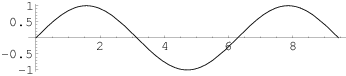
\includegraphics[width=8.5cm]{image1.png}}
%  \vspace{2.0cm}
  \centerline{(a) Result 1}\medskip
\end{minipage}
%
\begin{minipage}[b]{.48\linewidth}
  \centering
  \centerline{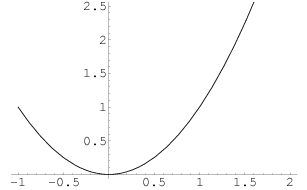
\includegraphics[width=4.0cm]{image3.png}}
%  \vspace{1.5cm}
  \centerline{(b) Results 3}\medskip
\end{minipage}
\hfill
\begin{minipage}[b]{0.48\linewidth}
  \centering
  \centerline{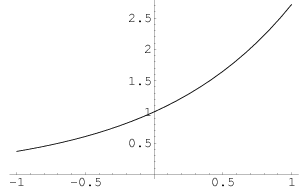
\includegraphics[width=4.0cm]{image4.png}}
%  \vspace{1.5cm}
  \centerline{(c) Result 4}\medskip
\end{minipage}
%
\caption{Example of placing a figure with experimental results.}
\label{fig:res}
%
\end{figure}


% To start a new column (but not a new page) and help balance the last-page
% column length use \vfill\pagebreak.
% -------------------------------------------------------------------------
%\vfill
%\pagebreak

\section{COPYRIGHT FORMS}
\label{sec:copyright}

You must include your fully completed, signed IEEE copyright release form when
form when you submit your paper. We {\bf must} have this form before your paper
can be published in the proceedings.

\section{REFERENCES}
\label{sec:ref}

List and number all bibliographical references at the end of the
paper. The references can be numbered in alphabetic order or in
order of appearance in the document. When referring to them in
the text, type the corresponding reference number in square
brackets as shown at the end of this sentence \cite{C2}. An
additional final page (the fifth page, in most cases) is
allowed, but must contain only references to the prior
literature.

% References should be produced using the bibtex program from suitable
% BiBTeX files (here: strings, refs, manuals). The IEEEbib.bst bibliography
% style file from IEEE produces unsorted bibliography list.
% -------------------------------------------------------------------------
\bibliographystyle{IEEEbib}
\bibliography{strings,refs}

\end{document}
